\documentclass{beamer}
\beamertemplatenavigationsymbolsempty
\usepackage[french]{babel}
\usepackage{fontspec}
\usepackage{amsmath, amsthm, amsfonts}
\usepackage[separate-uncertainty]{siunitx}
\usepackage{xcolor}
\usepackage{tikz}
\usepackage{tikz-cd}
\usepackage[object=vectorian]{pgfornament}
\usepackage{circuitikz}
\usepackage{hyperref}
\usepackage{caption}
\usepackage{booktabs}
\usepackage{mathtools}
\usepackage{longtable}
\usepackage[version=3]{mhchem}
\usepackage{marginnote}
\usepackage[framemethod=tikz]{mdframed}


% Paul Tol's qualitative palette
% ``bright''.https://personal.sron.nl/~pault/#sec:qualitative
\definecolor{tblue}{HTML}{4477AA}
\definecolor{tcyan}{HTML}{66CCEE}
\definecolor{tgreen}{HTML}{228833}
\definecolor{tyellow}{HTML}{CCBB44}
\definecolor{tred}{HTML}{EE6677}
\definecolor{tpurple}{HTML}{AA3377}
\definecolor{tgrey}{HTML}{BBBBBB}


% Justification for marginnotes.
\renewcommand*{\raggedleftmarginnote}{}
\renewcommand*{\raggedrightmarginnote}{}


% Styles for mdframed environments.
\newmdenv[backgroundcolor=tgreen!10,linecolor=tgreen!30]{reponsebox}
\newmdenv[backgroundcolor=tyellow!10,linecolor=tyellow!30]{diapobox}
\newmdenv[backgroundcolor=tred!10,linecolor=tred!30]{fondamentalbox}

% Default arrow for tikz and style for positive and negative objects.
\tikzset{>=latex,
    negative/.style={draw=teal!70!black, fill=teal!10, thick},
    positive/.style={draw=red, fill=red!10, thick}}
\usetikzlibrary{matrix,calc,decorations.pathreplacing,decorations.pathmorphing,decorations.markings}

% French locale for numbers and negative exponent for units.
\sisetup{locale=FR, per-mode=symbol}

\newcommand{\abs}[1]{\left| #1 \right|}
\newcommand{\rhat}{\vec{\hat{r}}}
\newcommand{\xhat}{\vec{\imath}}
\newcommand{\yhat}{\vec{\jmath}}
\newcommand{\zhat}{\vec{k}}
\newcommand{\real}{\mathbb{R}}
\newcommand{\der}[2]{\frac{\mathrm{d}#1}{\mathrm{d}#2}}
\newcommand{\pder}[2]{\frac{\partial\ #1}{\partial\ #2}}
\newcommand{\dif}{\mathrm{d}}
\newcommand{\ddif}{\,\mathrm{d}}
\newcommand{\grad}{\vec{\nabla}}
\newcommand{\exemple}[1]{\begin{fullwidth}#1\end{fullwidth}}
\newcommand{\norm}[1]{\lVert\ #1\ \rVert}
\newcommand{\vu}{\vec{u}}
\newcommand{\vv}{\vec{v}}
\newcommand{\vr}{\vec{r}}
\newcommand{\va}{\vec{a}}
\newcommand{\vF}{\vec{F}}
\newcommand{\vE}{\vec{E}}
\newcommand{\vB}{\vec{B}}
\newcommand{\vecxyz}[3]{#1 \xhat\ + #2 \yhat\ + #3 \zhat}
\newcommand{\vecxy}[2]{#1 \xhat\ + #2 \yhat}
\newcommand{\coulombcst}{k}
\newcommand{\emf}{\ensuremath{\mathcal{E}}}
\newcommand{\eval}{\SI{1.602e-19}{C}}
\newcommand{\kval}{\SI{8.99e9}{Nm^2 \per C^2}}

% Nice separator line
\newcommand{\sectionline}{
    \noindent
    \begin{center}
        \resizebox{0.5\linewidth}{1ex}
    {{%
    {\begin{tikzpicture}
    \node  (C) at (0,0) {};
    \node (D) at (9,0) {};
    \path (C) to [ornament=85] (D);
    \end{tikzpicture}}}}
    \end{center}
}

\theoremstyle{definition}
\newtheorem*{defn}{Definition}


\usepackage[version=3]{mhchem}

\setbeamercolor{title}{fg=tblue}
\setbeamercolor{frametitle}{fg=tblue}
\setbeamercolor{structure}{fg=tblue}

% Make footnotesize smaller
\makeatletter
\renewcommand\footnotesize{%
   \@setfontsize\footnotesize\@viipt{11}%
   \abovedisplayskip 8\p@ \@plus2\p@ \@minus4\p@
   \abovedisplayshortskip \z@ \@plus\p@
   \belowdisplayshortskip 4\p@ \@plus2\p@ \@minus2\p@
   \def\@listi{\leftmargin\leftmargini
               \topsep 4\p@ \@plus2\p@ \@minus2\p@
               \parsep 2\p@ \@plus\p@ \@minus\p@
               \itemsep \parsep}%
   \belowdisplayskip \abovedisplayskip
}
\makeatother

\title{Électricité et magnétisme}
\subtitle{Chapitre 4 - Potentiel électrique}
\date{21 septembre 2021}
\author{Loïc Séguin-Charbonneau}
\institute{Cégep Édouard-Montpetit}

\begin{document}

\maketitle


\begin{frame}[t]{Travail effectué par la force électrique}

Classez les situations suivantes en ordre croissant du travail fait par la
force électrique sur la charge $q > 0$.

\begin{center}
  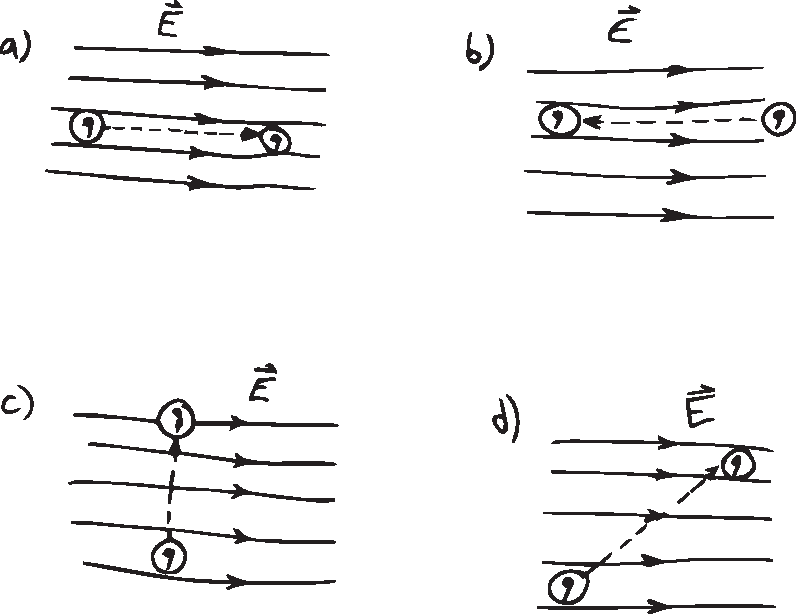
\includegraphics[scale=0.6]{figures/travail-force-electrique.pdf}
\end{center}

\end{frame}


%\begin{frame}[t]{Est-ce que la force électrique est conservative?}

%Une particule de déplace de l'origine $\vec{r}_0 = \vecxyz{0}{0}{0}$ jusqu'au
%point $\vec{r} = \vecxyz{a}{b}{c}$ dans un champ électrique constant $\vec{E} =
%E_z \zhat$ où $E_z$ est constant.

%Déterminer le travail fait par la force électrique pour les deux trajectoires
%suivantes.

%\begin{itemize}
  %\item Le long de la ligne droite qui relie $\vec{r}_0$ à $\vec{r}$.
  %\item Le long de la ligne qui va de $\vec{r}_0$ à $\vecxyz{a}{b}{0}$, puis le
    %long de la ligne qui va de $\vecxyz{a}{b}{0}$ à $\vecxyz{a}{b}{c}$.
%\end{itemize}

%\end{frame}

\begin{frame}{Charge ponctuelle dans un champ uniforme}
  On place une charge ponctuelle positive au-dessus d'une grande plaque chargée
  positivement. Si on approche la charge ponctuelle de la plaque, lequel des
  énoncés est vrai?

  \begin{center}
    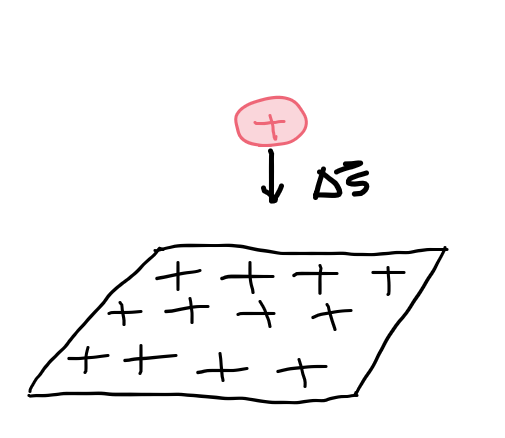
\includegraphics[width=0.3\textwidth]{figures/charge_dessus_plaque_approche.png}
  \end{center}

  \begin{enumerate}[A.]
    \item La force électrique fait un travail positif.
    \item La force électrique ne fait aucun travail.
    \item<alert@2> L'énergie potentielle du système augmente.
    \item L'énergie potentielle du système diminue.
  \end{enumerate}

\end{frame}


\begin{frame}{Charge ponctuelle dans un champ uniforme}
  On place une charge ponctuelle positive au-dessus d'une grande plaque chargée
  positivement. Si on éloigne la charge ponctuelle de la plaque, lequel des
  énoncés est vrai?

  \begin{center}
    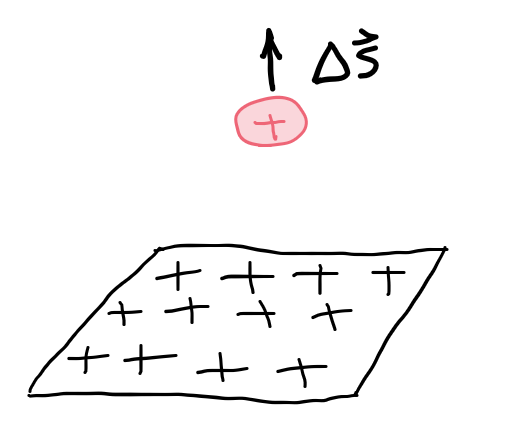
\includegraphics[width=0.3\textwidth]{figures/charge_dessus_plaque_eloigne.png}
  \end{center}

  \begin{enumerate}[A.]
    \item<alert@2> La force électrique fait un travail positif.
    \item La force électrique ne fait aucun travail.
    \item L'énergie potentielle du système augmente.
    \item<alert@2> L'énergie potentielle du système diminue.
  \end{enumerate}

\end{frame}


\begin{frame}[t]{Charge ponctuelle dans un champ uniforme}
  Une particule de charge \SI{-8.00}{\micro\coulomb} est placée
  \SI{2.00}{\meter} à gauche d'une grande plaque verticale portant une charge
  surfacique de \SI{50.0}{\nano\coulomb\per\meter\squared}. La particule
  s'approche de \SI{1.00}{\meter} de la plaque. Elle a une masse de
  \SI{0.200}{\milli\gram}.

  \vspace{\baselineskip}

  \begin{columns}[t]
    \column{0.6\textwidth}

    \only<1-2>{
      Le travail fait par la force électrique est

      \begin{enumerate}[A.]
        \item<alert@2> Positif
        \item Négatif
        \item Nul
      \end{enumerate}
    }

    \only<3-4>{
      L'énergie potentielle du système

      \begin{enumerate}[A.]
        \item Augmente
        \item<alert@4> Diminue
        \item Ne change pas
      \end{enumerate}
    }

    \only<5-6>{
      Si aucun travail externe n'est effectué, l'énergie cinétique de la
      particule

      \begin{enumerate}[A.]
        \item<alert@6> Augmente
        \item Diminue
        \item Ne change pas
      \end{enumerate}
    }

    \only<7>{
      Quel est le travail effectué par la force électrique?
    }

    \only<8>{
      Quel est la variation d'énergie potentielle électrique?
    }

    \only<9>{
      Si aucun travail externe n'est effectué et que la particule était
      initialement au repos, quelle est sa vitesse à la fin de son mouvement?
    }

    \column{0.3\textwidth}
    \begin{center}
      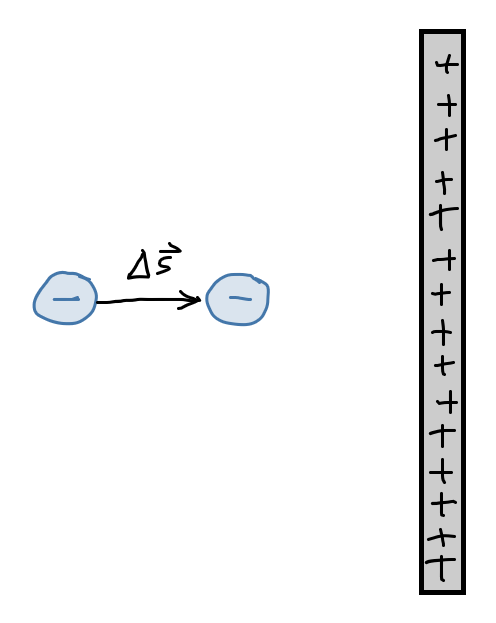
\includegraphics[width=\textwidth]{figures/charge_neg_gauche_plaque.png}
    \end{center}
  \end{columns}
\end{frame}



\begin{frame}[t]{Atome d'hydrogène}
  Un atome d'hydrogène est constitué d'un électron et d'un proton. On
  assemble un atome d'hydrogène à partir d'un électron et d'un proton isolé
  qu'on approche jusqu'à une distance de \SI{1.06e-10}{\meter}. Si on pose que
  l'énergie potentielle du système est nulle lorsque les deux particules sont
  isolées, quelle est l'énergie potentielle de l'atome d'hydrogène assemblé?
  \begin{center}
    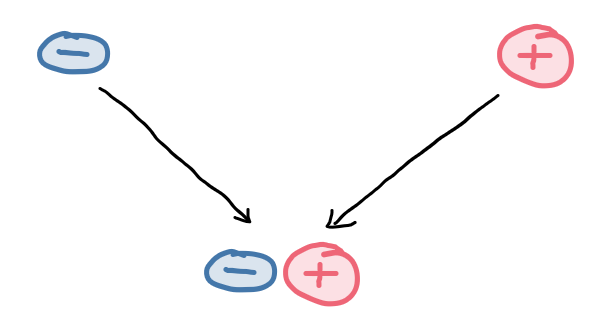
\includegraphics[width=0.5\textwidth]{figures/hydrogene.png}
  \end{center}
\end{frame}


%\begin{frame}[t]{Exemple}

%On considère une mince tige métallique cylindrique très longue portant une
%charge uniforme.  La densité linéique de charge est de $\lambda =
%\SI{0.948}{\micro\coulomb\per\meter}$. Un électron est relâché \SI{35}{mm}
%de la tige.

%\begin{enumerate}
  %\item Calculer la variation d'énergie potentielle du système après que
    %l'électron se soit déplacé de \SI{1}{cm}.
  %\item Si l'électron était initialement au repos, déterminer sa vitesse à la
    %fin de son déplacement.
  %\item Tracer un graphique du module du champ électrique généré par la tige en
    %fonction de la distance par rapport à son axe.
  %\item Tracer un graphique de l'énergie potentielle de l'électron en fonction
    %de sa distance par rapport à l'axe de la tige.
%\end{enumerate}

%\end{frame}


\begin{frame}[t]{Différence de potentiel et potentiel}
  \begin{center}
    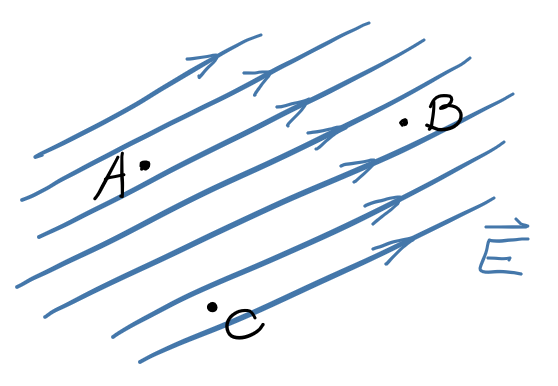
\includegraphics[width=0.5\textwidth]{figures/vbva.png}
  \end{center}

  \only<1-2>{
    La différence de potentiel lorsqu'on passe de A à B est

    \begin{enumerate}[A.]
      \item positive
      \item<alert@2> négative
      \item nulle
    \end{enumerate}
  }

  \only<3-4>{
    On peut donc conclure que le potentiel en A est

    \begin{enumerate}[A.]
      \item<alert@4> plus grand que le potentiel en B
      \item plus petit que le potentiel en B
      \item identique au potentiel en B
    \end{enumerate}
  }

  \only<5-6>{
    Le potentiel est donc plus grand
    \begin{enumerate}[A.]
      \item<alert@6> près des charges positives
      \item près des charges négatives
      \item lorsqu'il neige
    \end{enumerate}
  }

  \only<7-8>{
    La différence de potentiel lorsqu'on passe de A à C est

    \begin{enumerate}[A.]
      \item positive
      \item négative
      \item<alert@8> nulle
    \end{enumerate}
  }

  \only<9-10>{
    On peut donc conclure que le potentiel en A est

    \begin{enumerate}[A.]
      \item plus grand que le potentiel en C
      \item plus petit que le potentiel en C
      \item<alert@10> identique au potentiel en C
    \end{enumerate}
  }

  \only<11-12>{
    Si la différence de potentiel lorsqu'on passe de A à B est de \SI{-15}{V},
    quelle est la différence de potentiel lorsqu'on passe de B à A?

    \begin{enumerate}[A.]
      \item<alert@12> \SI{15}{V}
      \item \SI{-15}{V}
      \item impossible à déterminer sans la valeur du champ électrique
    \end{enumerate}
  }

  \only<13-14>{
    Parmi les choix suivants, un seul donne des valeurs de potentiel aux points
    A, B et C cohérentes avec le dessin.

    \begin{enumerate}[A.]
      \item $V_A = \SI{15}{V}, V_B = \SI{30}{V}, V_C = \SI{15}{V}$
      \item $V_A = \SI{15}{V}, V_B = \SI{0}{V}, V_C = \SI{0}{V}$
      \item<alert@14> $V_A = \SI{-15}{V}, V_B = \SI{-30}{V}, V_C = \SI{-15}{V}$
      \item $V_A = \SI{-45}{V}, V_B = \SI{-30}{V}, V_C = \SI{45}{V}$
    \end{enumerate}
  }
\end{frame}

\begin{frame}{Électron entre deux plaques}

Deux grandes plaques métalliques sont maintenues à une différence de potentiel
de \SI{12}{V}. Elles sont séparées d'une distance de \SI{1}{cm}. Un électron
qui se trouve juste à côté d'une des plaques se déplace jusqu'à l'autre plaque.
Si l'électron est initialement immobile, déterminer le module de sa vitesse
lorsqu'il atteint l'autre plaque.

\end{frame}



\begin{frame}{Deux plaques qu'on éloigne}

Deux grandes plaques métalliques sont maintenues à une différence de potentiel
de \SI{12}{V}. On augmente la distance entre les plaques. Expliquez ce qui doit
se produire avec la densité surfacique de charge sur les plaques pour que la
différence de potentiel demeure constante.

\end{frame}



\begin{frame}{Exercice équipotentielles}
On place un électron dans une région de l'espace où les surfaces
équipotentielles sont telles qu'illustrées dans le schéma ci-dessous.

\begin{center}
  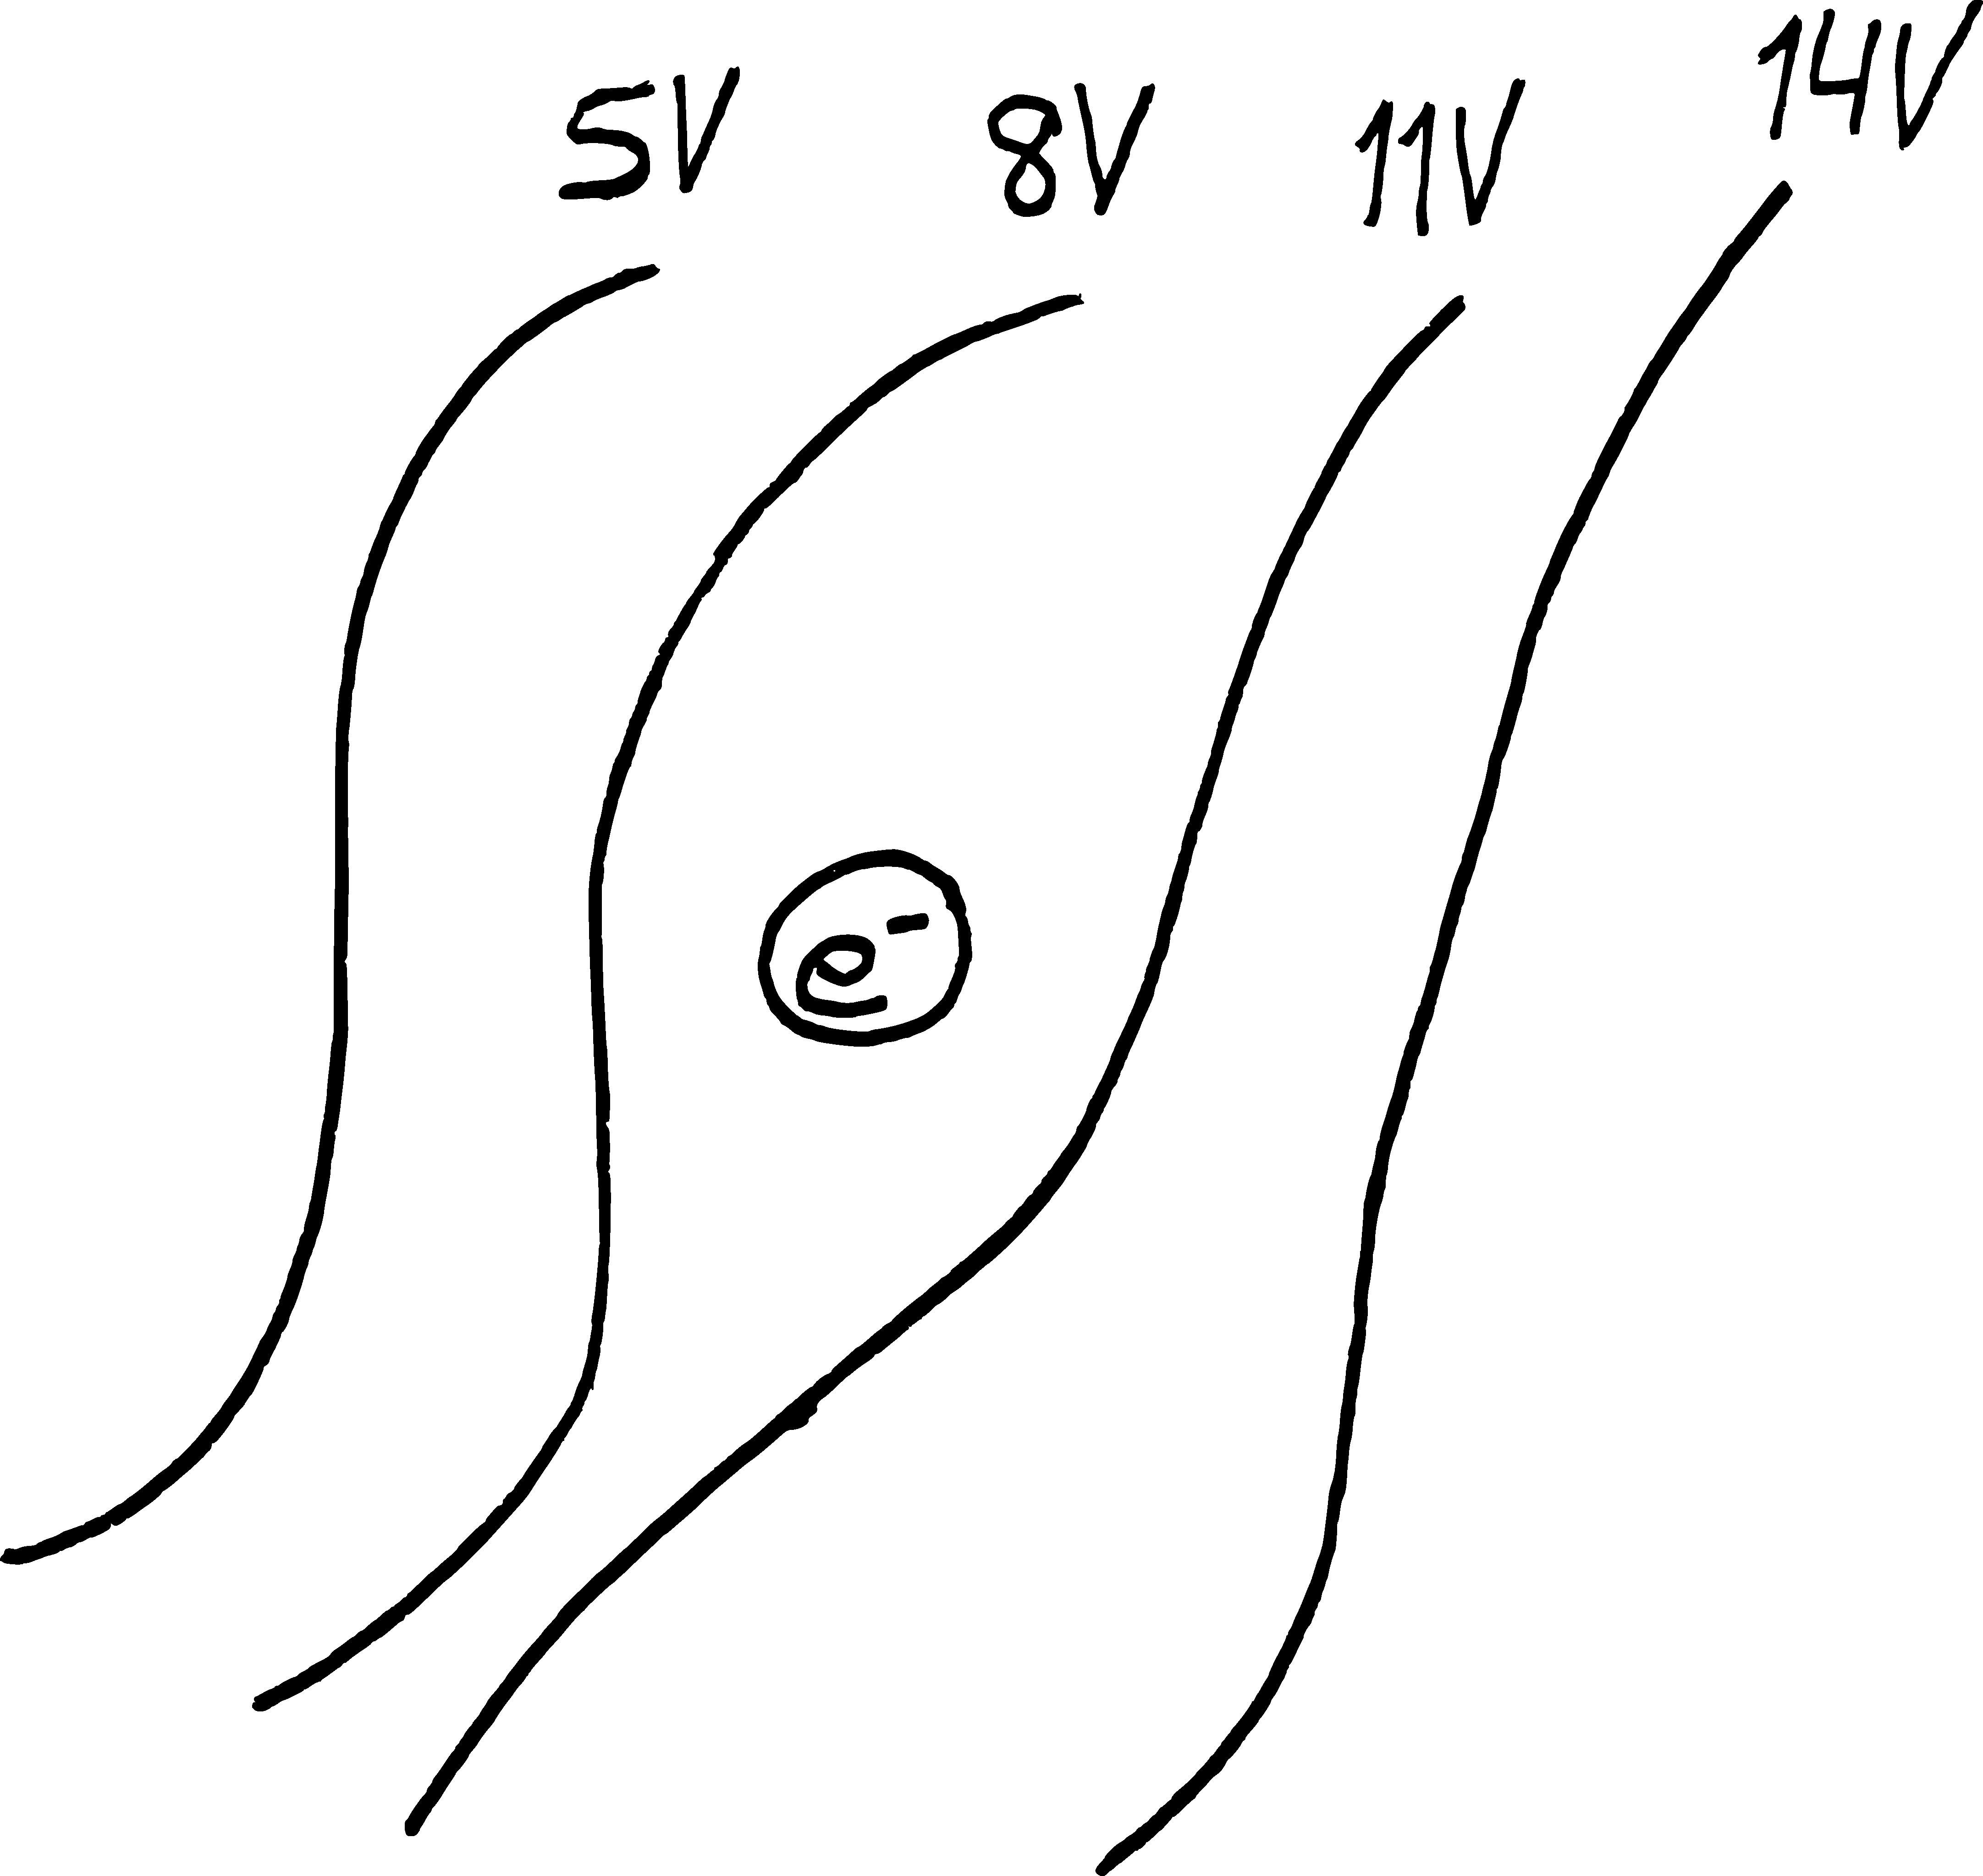
\includegraphics[width=5cm]{figures/exercice-equipotentielles.pdf}
\end{center}

\begin{enumerate}
  \item Dans quelle direction est la force que subit l'électron?
  \item Tracez les lignes de champ électrique.
\end{enumerate}
\end{frame}



\begin{frame}{Énergie potentielle de charges ponctuelles}

Trois charges sont placées aux sommets d'un carré de côté $d = \SI{3}{cm}$. Les
charges sont de $q_1 = \SI{1.7}{\micro\coulomb}$, $q_2 = \SI{-3}{\micro\coulomb}$,
et $q_3 = \SI{2}{\micro\coulomb}$.


\begin{itemize}
  \item Déterminer le potentiel au point $P$, \SI{3}{cm} au-dessus de la
    charge $q_1$.
  \item On amène une charge $q_4 = \SI{-4}{\micro\coulomb}$ de l'infini jusqu'à $P$.
    Quel est le changement d'énergie potentielle du système? Que signifie la
    réponse?
\end{itemize}

\begin{center}
  \begin{tikzpicture}
    \coordinate (p1) at (0, 0);
    \coordinate (p2) at (2, 0);
    \coordinate (p3) at (2, 2);
    \coordinate (p4) at (0, 2);
    \node[draw, circle] (q1) at (p1) {$q_1$};
    \node[draw, circle] (q2) at (p2) {$q_2$};
    \node[draw, circle] (q3) at (p3) {$q_3$};
    %\node[draw, circle] (q4) at (p4) {$q_4$};
    \fill (p4) circle (2pt);
    \node[anchor=south east] at (p4) {$P$};
    \draw[<->] (q1) -- node[fill=white] {$d$} (q2);
    \draw[<->] (q2) -- node[fill=white] {$d$} (q3);
    \draw[dashed] (q1) -- (p4);
    \draw[dashed] (q3) -- (p4);
  \end{tikzpicture}
\end{center}
\end{frame}


\end{document}
